
\documentclass[conference]{IEEEtran}
% Some Computer Society conferences also require the compsoc mode option,
% but others use the standard conference format.
%
% If IEEEtran.cls has not been installed into the LaTeX system files,
% manually specify the path to it like:
% \documentclass[conference]{../sty/IEEEtran}





% Some very useful LaTeX packages include:
% (uncomment the ones you want to load)



% *** SOME SELECTED PACKAGES ***
%
\usepackage{cite}


\usepackage{amsmath}								% Use math symbols
\usepackage{amssymb}								% Defines symbols in AMS symbol fonts msam and msbm
\usepackage{commath}                                % Gives you \dif for the differential in an integral
\newcommand{\brkt}[1]{\langle #1 \rangle}
\DeclareMathOperator{\Expectation}{\mathbb{E}}
\DeclareMathOperator{\Variance}{Var}
\DeclareMathOperator{\Covariance}{Cov}

\DeclareMathOperator{\BesselJfn}{J}   % Bessel First Kind
\DeclareMathOperator{\BesselYfn}{Y}   % Bessel Second Kind

\DeclareMathOperator{\StruveFn}{\mathbf{H}}   % Struve function

\DeclareMathOperator{\sinc}{sinc}

\newcommand{\E}[1]{\Expectation\lbrack#1\rbrack}
\newcommand{\Var}[1]{\Variance\lbrack#1\rbrack}
\newcommand{\Cov}[2]{\Covariance\lbrack#1,#2\rbrack}
\newcommand{\BesselJ}[2]{\BesselJfn_{#1}(#2)}
\newcommand{\BesselY}[2]{\BesselYfn_{#1}(#2)}
\newcommand{\StruveH}[2]{\StruveFn_{#1}(#2)}
\newcommand{\xbar}{\bar{\chi}}

\usepackage[dvipsnames]{xcolor}
\newcommand{\bfr}[1]{\textbf{\color{BrickRed} #1}}

\hyphenation{
im-ped-ance back-scat-ter-ing Som-mer-feld-Wat-son
} 

\usepackage{cite}									% Improves normal latex citation mechanism when handling numeric citations

\usepackage{nicefrac}                               % Gives you the ability to make inline fractions
\usepackage{pdfsync}                                % Enables synchronization between text editor and pdf viewer
\usepackage{units}                                  % Proper typesetting of units

\usepackage[pdftex]{graphicx}
% declare the path(s) where your graphic files are
\graphicspath{{../output/}}
% and their extensions so you won't have to specify these with
% every instance of \includegraphics
\DeclareGraphicsExtensions{.pdf,.jpeg,.png,.eps}

\usepackage{epstopdf}								% Converts .eps figures to pdf format


% *** SUBFIGURE PACKAGES ***
\ifCLASSOPTIONcompsoc
  \usepackage[caption=false,font=normalsize,labelfont=sf,textfont=sf]{subfig}
\else
  \usepackage[caption=false,font=footnotesize]{subfig}
\fi
% subfig.sty, written by Steven Douglas Cochran, is the modern replacement
% for subfigure.sty, the latter of which is no longer maintained and is
% incompatible with some LaTeX packages including fixltx2e. However,
% subfig.sty requires and automatically loads Axel Sommerfeldt's caption.sty
% which will override IEEEtran.cls' handling of captions and this will result
% in non-IEEE style figure/table captions. To prevent this problem, be sure
% and invoke subfig.sty's "caption=false" package option (available since
% subfig.sty version 1.3, 2005/06/28) as this is will preserve IEEEtran.cls
% handling of captions.
% Note that the Computer Society format requires a larger sans serif font
% than the serif footnote size font used in traditional IEEE formatting
% and thus the need to invoke different subfig.sty package options depending
% on whether compsoc mode has been enabled.
%
% The latest version and documentation of subfig.sty can be obtained at:
% http://www.ctan.org/pkg/subfig




% *** FLOAT PACKAGES ***
%
%\usepackage{fixltx2e}
% fixltx2e, the successor to the earlier fix2col.sty, was written by
% Frank Mittelbach and David Carlisle. This package corrects a few problems
% in the LaTeX2e kernel, the most notable of which is that in current
% LaTeX2e releases, the ordering of single and double column floats is not
% guaranteed to be preserved. Thus, an unpatched LaTeX2e can allow a
% single column figure to be placed prior to an earlier double column
% figure.
% Be aware that LaTeX2e kernels dated 2015 and later have fixltx2e.sty's
% corrections already built into the system in which case a warning will
% be issued if an attempt is made to load fixltx2e.sty as it is no longer
% needed.
% The latest version and documentation can be found at:
% http://www.ctan.org/pkg/fixltx2e


%\usepackage{stfloats}
% stfloats.sty was written by Sigitas Tolusis. This package gives LaTeX2e
% the ability to do double column floats at the bottom of the page as well
% as the top. (e.g., "\begin{figure*}[!b]" is not normally possible in
% LaTeX2e). It also provides a command:
%\fnbelowfloat
% to enable the placement of footnotes below bottom floats (the standard
% LaTeX2e kernel puts them above bottom floats). This is an invasive package
% which rewrites many portions of the LaTeX2e float routines. It may not work
% with other packages that modify the LaTeX2e float routines. The latest
% version and documentation can be obtained at:
% http://www.ctan.org/pkg/stfloats
% Do not use the stfloats baselinefloat ability as the IEEE does not allow
% \baselineskip to stretch. Authors submitting work to the IEEE should note
% that the IEEE rarely uses double column equations and that authors should try
% to avoid such use. Do not be tempted to use the cuted.sty or midfloat.sty
% packages (also by Sigitas Tolusis) as the IEEE does not format its papers in
% such ways.
% Do not attempt to use stfloats with fixltx2e as they are incompatible.
% Instead, use Morten Hogholm'a dblfloatfix which combines the features
% of both fixltx2e and stfloats:
%
% \usepackage{dblfloatfix}
% The latest version can be found at:
% http://www.ctan.org/pkg/dblfloatfix




% *** PDF, URL AND HYPERLINK PACKAGES ***
%
%\usepackage{url}
% url.sty was written by Donald Arseneau. It provides better support for
% handling and breaking URLs. url.sty is already installed on most LaTeX
% systems. The latest version and documentation can be obtained at:
% http://www.ctan.org/pkg/url
% Basically, \url{my_url_here}.




% *** Do not adjust lengths that control margins, column widths, etc. ***
% *** Do not use packages that alter fonts (such as pslatex).         ***
% There should be no need to do such things with IEEEtran.cls V1.6 and later.
% (Unless specifically asked to do so by the journal or conference you plan
% to submit to, of course. )


% correct bad hyphenation here
\hyphenation{op-tical net-works semi-conduc-tor}


\begin{document}
%
% paper title
% Titles are generally capitalized except for words such as a, an, and, as,
% at, but, by, for, in, nor, of, on, or, the, to and up, which are usually
% not capitalized unless they are the first or last word of the title.
% Linebreaks \\ can be used within to get better formatting as desired.
% Do not put math or special symbols in the title.
\title{[DRAFT IN PROGRESS] Managing Irritable Bowel Syndrome Through Lightweight, Daily Tracking}


% author names and affiliations
% use a multiple column layout for up to three different
% affiliations
\author{\IEEEauthorblockN{Isaac D. Gerg, TODO }
\IEEEauthorblockA{The Pennsylvania State Univeristy\\
Applied Research Laboratory\\
State College, PA 16804--0030\\
Email: idg101@arl.psu.edu}
}

% conference papers do not typically use \thanks and this command
% is locked out in conference mode. If really needed, such as for
% the acknowledgment of grants, issue a \IEEEoverridecommandlockouts
% after \documentclass




% make the title area
\maketitle

% As a general rule, do not put math, special symbols or citations
% in the abstract
\begin{abstract}
Irttiable bowel syndrome (IBS) is a multifaceted syndrome with generally unknown etiology with few exceptions [pimentel cite].  It primarily manifests itself through one or more symptoms of chronic diarrhea, constipation, and abdominal pain.  Generally, it is a diagnosis of exclusion after the patient has had a comprehensive workup. In this paper, we show how the author, the patient, who is a 34 year old male diagnosed with irritable bowel syndrome  manifesting through symptoms of abdominal pain and diarrhea, utilizes a smartphone application and spreadhseet to track bowel movements, medication, exercise, and overall functionality to assess treatment efficacy.
\end{abstract}

% no keywords



% For peer review papers, you can put extra information on the cover
% page as needed:
% \ifCLASSOPTIONpeerreview
% \begin{center} \bfseries EDICS Category: 3-BBND \end{center}
% \fi
%
% For peerreview papers, this IEEEtran command inserts a page break and
% creates the second title. It will be ignored for other modes.
\IEEEpeerreviewmaketitle



\section{Introduction}
% no \IEEEPARstart
IBS is a multifacieted syndrom witih generally unknown etiology with the exception of the recent work done by Rao and Pimentel.  Generally, patients go through a battery of tests and eventually IBS is diagnosed as moreso an exclusion of other, more life threatening conditions such as chrons diease or ulcerative colitis.   Depits TODO of US population diagnosed with IBS, treating it difficult.  Doctors and have many approaches to treatment which include anti-spasodmoics, cognitive behaviour therepy (CBT), altered diet [FODMPA citatpion], SSRIs, and TCAs. Anecdotal, doctors and patients generally use a “try-and-see” approach for symptom managagment akin to contemperorary SSRI managment [TODO stard trial].

In this study, we seek to quantify symptom serverity, bowel habits, and medications in a lightweight manner making daily compliance of record keeping easy and regress on the data to determine what treatments are effective for an N=1 study, i.e. the author.  There has been much overlap between eitologies of anxiety and depression with IBS [TODO citation] so there is a strong need to have objective eidence to support a particlarly treatement especially because the placebo effect [TODO cite kirch work] may be large and the side effect profile of many IBS treatments may add to the treatment themselves [TODO cite side effects of nexium and librax.]

\section{Tracking Methodology}

The patient uses a simple android applicatoin and google spreadsheet for daily tracking.  The android applicaoitn used is Bowel Move and requires a handful of clicks to enter a BM.  Likewise, google spreadsheets are available on most internet connected platforms and smart phones making it easy to find a suitable computer to enter in daily data.  Together, compliance of the record keeping protocol exceeds 99%.

The patient keeps log of the following items through a Google spreadsheet:

\begin{itemize}[noitemsep]
\item AM/PM Health Quality Index (HQI)
\item Medication intake as dosage
\item Time spent performing cardiovascular exercise
\item Body weight
\end{itemize}

HQI is defined on a 1-4 scale describing how the symptoms manifest themselves as a function of the patients ability to complete his daily wishes ans plans (e.g. work, exercise, time with family, etc).  HQI has defined levels which are:

\begin{enumerate}
  \item Symptom severity requires medical urgent medical attention (e.g. ED visit)
  \item Symptom severity prevents patient from completly daily wishes (e.g. missed a day of work due to persistant abdominal pain)
  \item Symptoms notable but patient is able to cope with symptoms to complete daily wishes (e.g. a stomach ache while at a baseball game which is tolerable and resolves with time)
  \item Symptoms are not present.
\end{enumerate}

Medications are recorded as total daily dose.  For example, a daily dose of 20mg Nexium bid is entered as 40mg. Time spent performing cardio recorded as total daily time in minutes.  For example, a two-hour mountain bike ride is records as 120 minutes. Daily weight is recorded first thing in the morning and entered in pounds.

\section{Data Visualization}

Bristol Stool Scores (BSS) over the sampling period are shown below.

\begin{figure}[t]
    \centering
    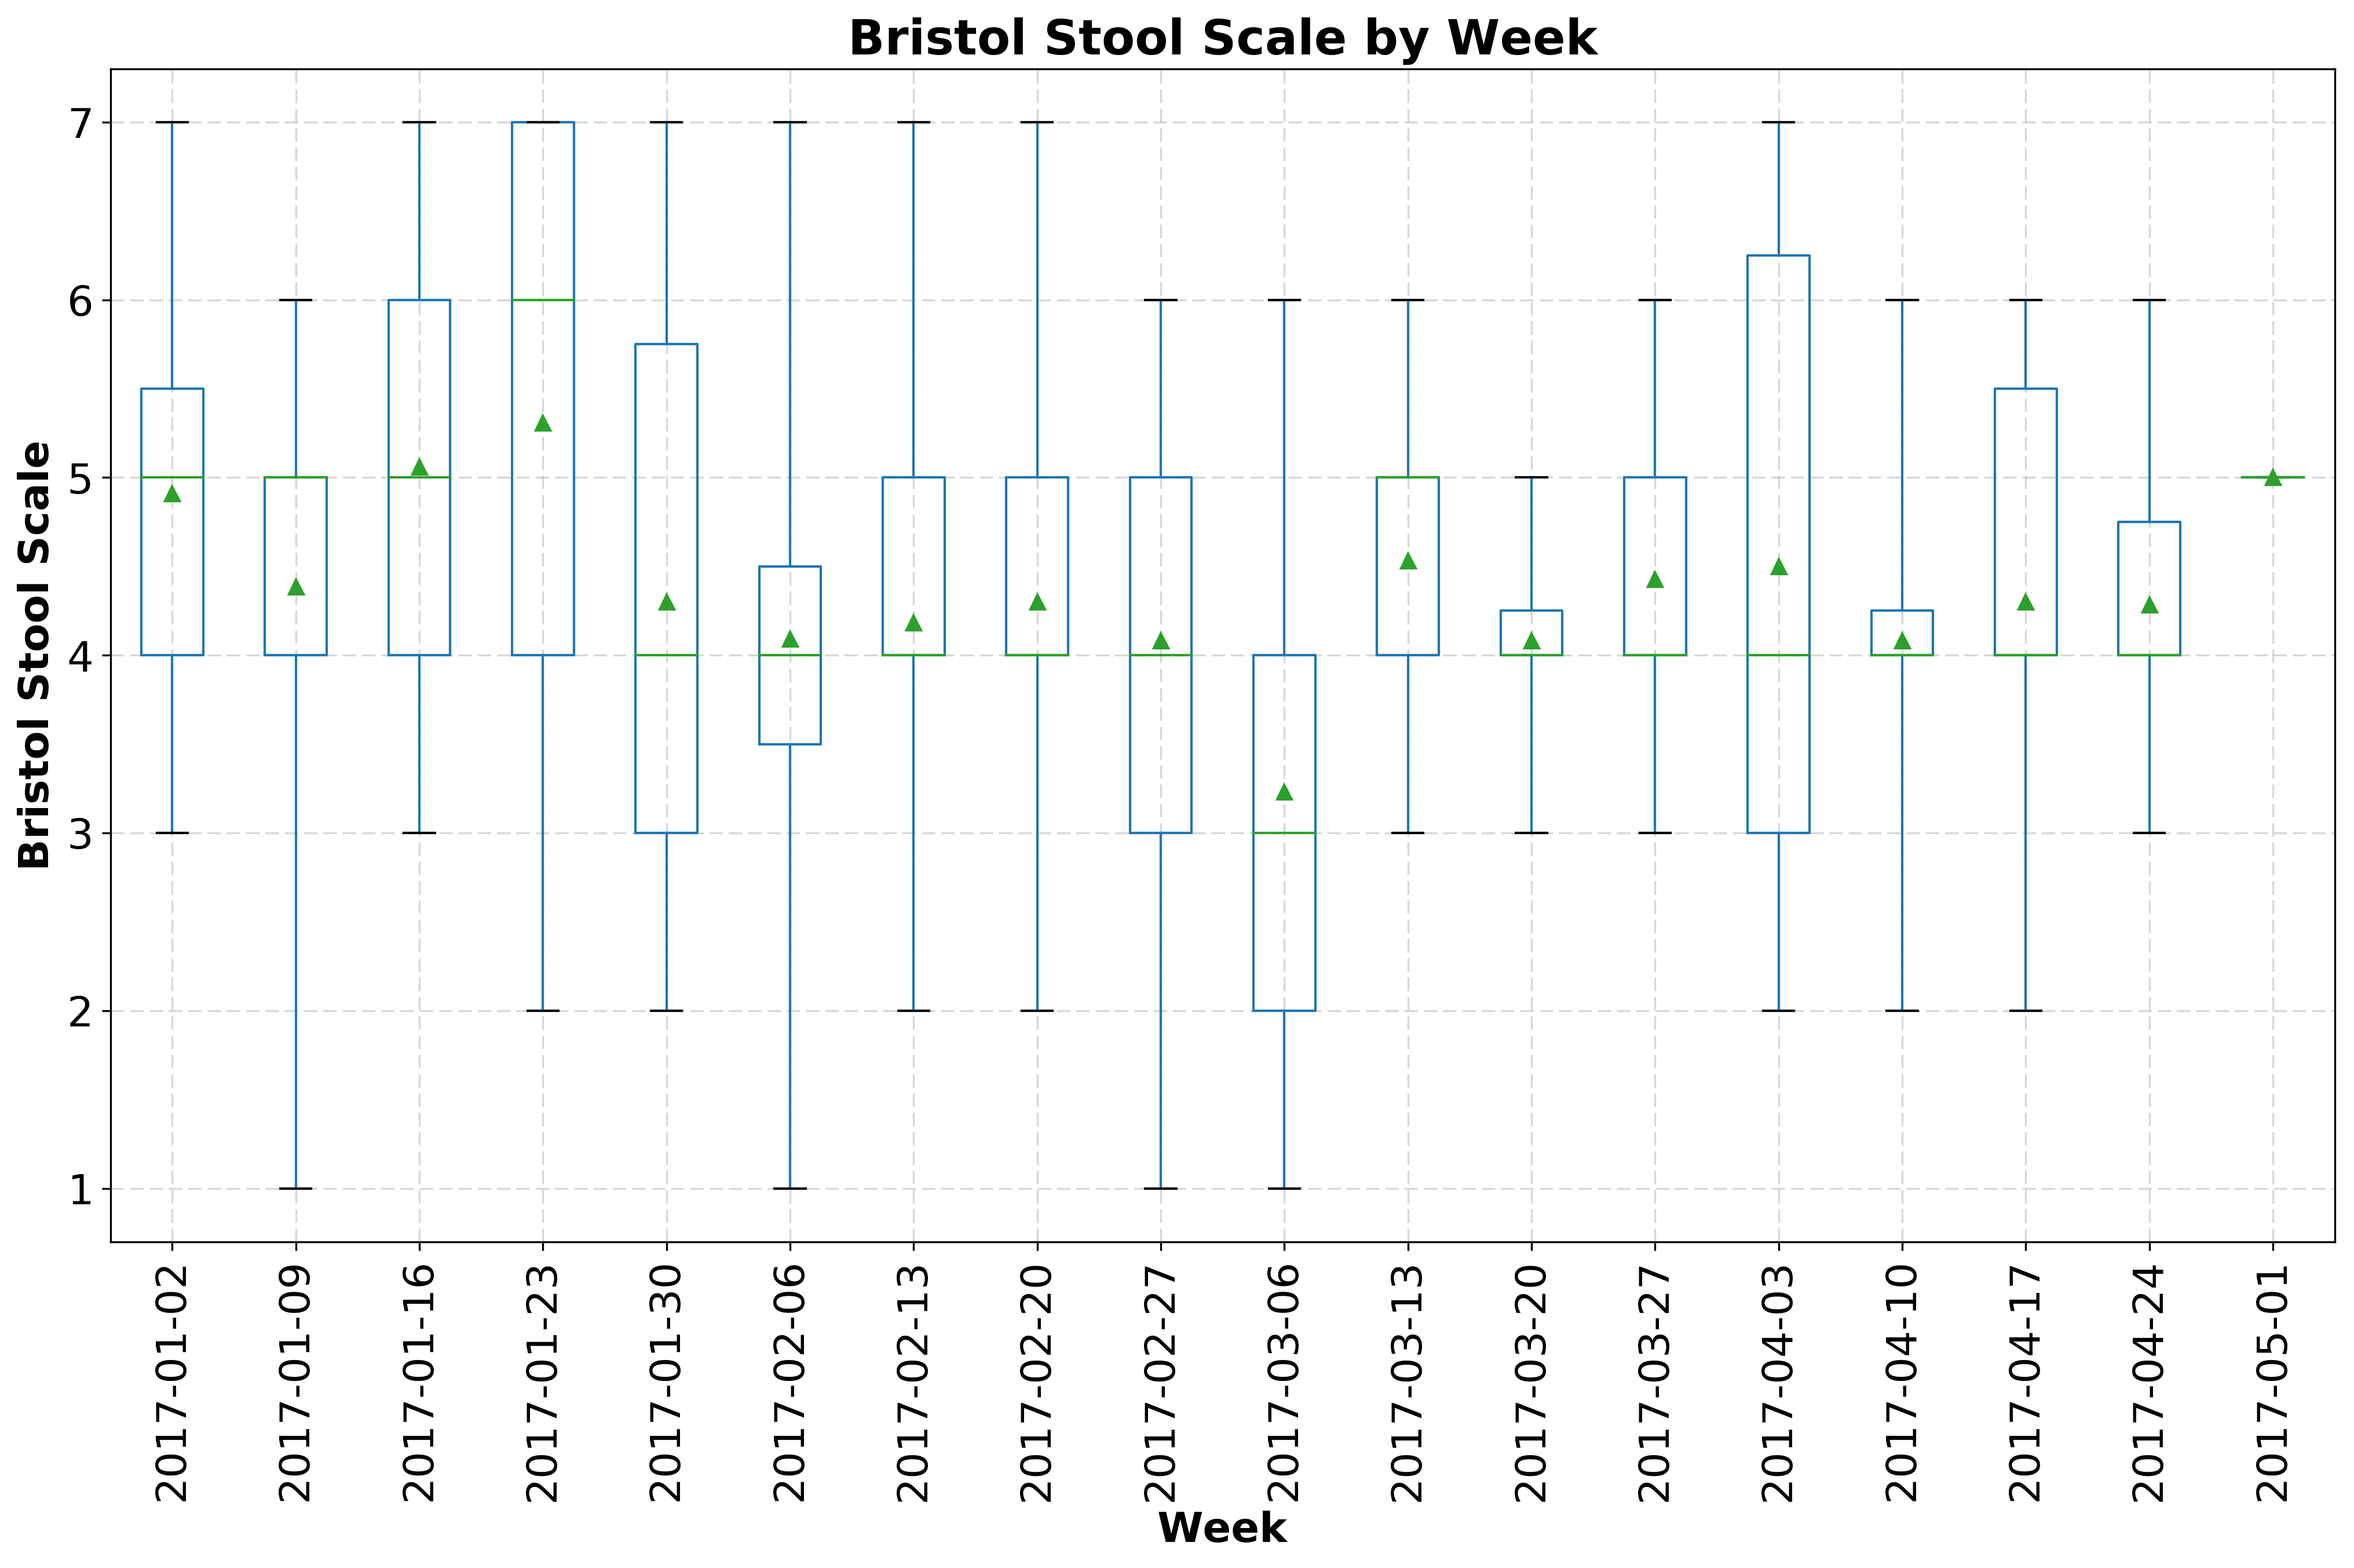
\includegraphics[width=\columnwidth]{bss_box_whisker.png}
    \caption{Bristol Stool Score by Week}\label{fig:bss_box_whisker}
\end{figure}

We are interested in the number of bowel movements outside the 3-5 BSS. We defines these as abnormal movements and wish to minimize their presence.  We show their contribution below.

\begin{figure}[t]
    \centering
    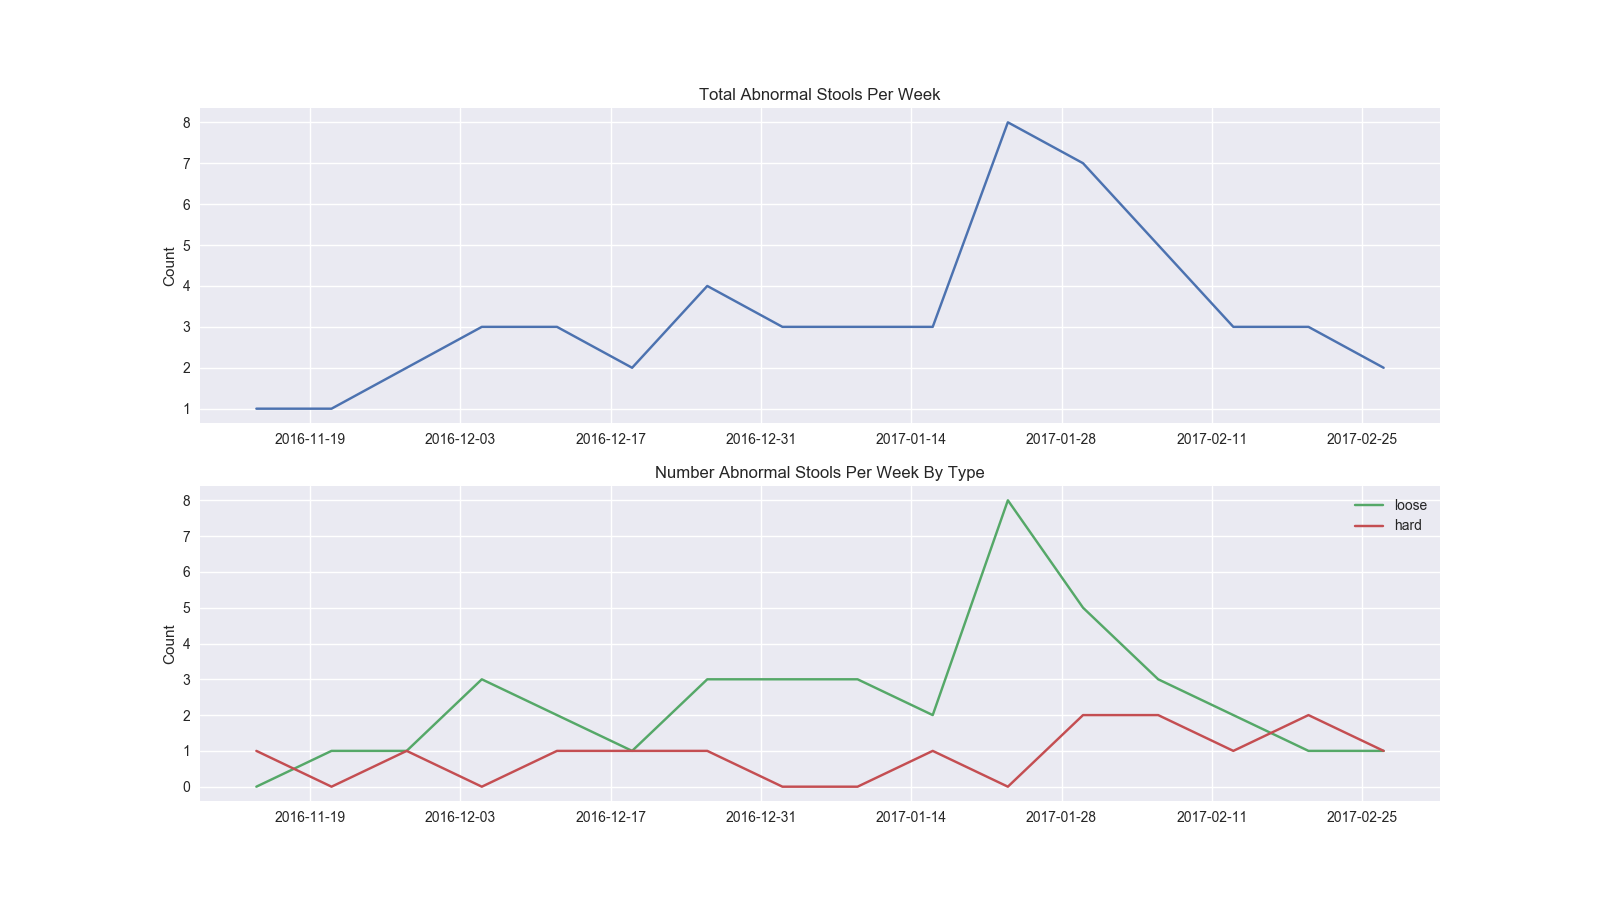
\includegraphics[width=\columnwidth]{abnormal.png}
    \caption{Abnormal Bowel Movements by Week and Type}\label{fig:bss_abnormal}
\end{figure}

The time between movements we list for completeness below.  The plot shows a bimodal distribution and the author believes the left-most peak is characteristic of IBS-D.

\begin{figure}[t]
    \centering
    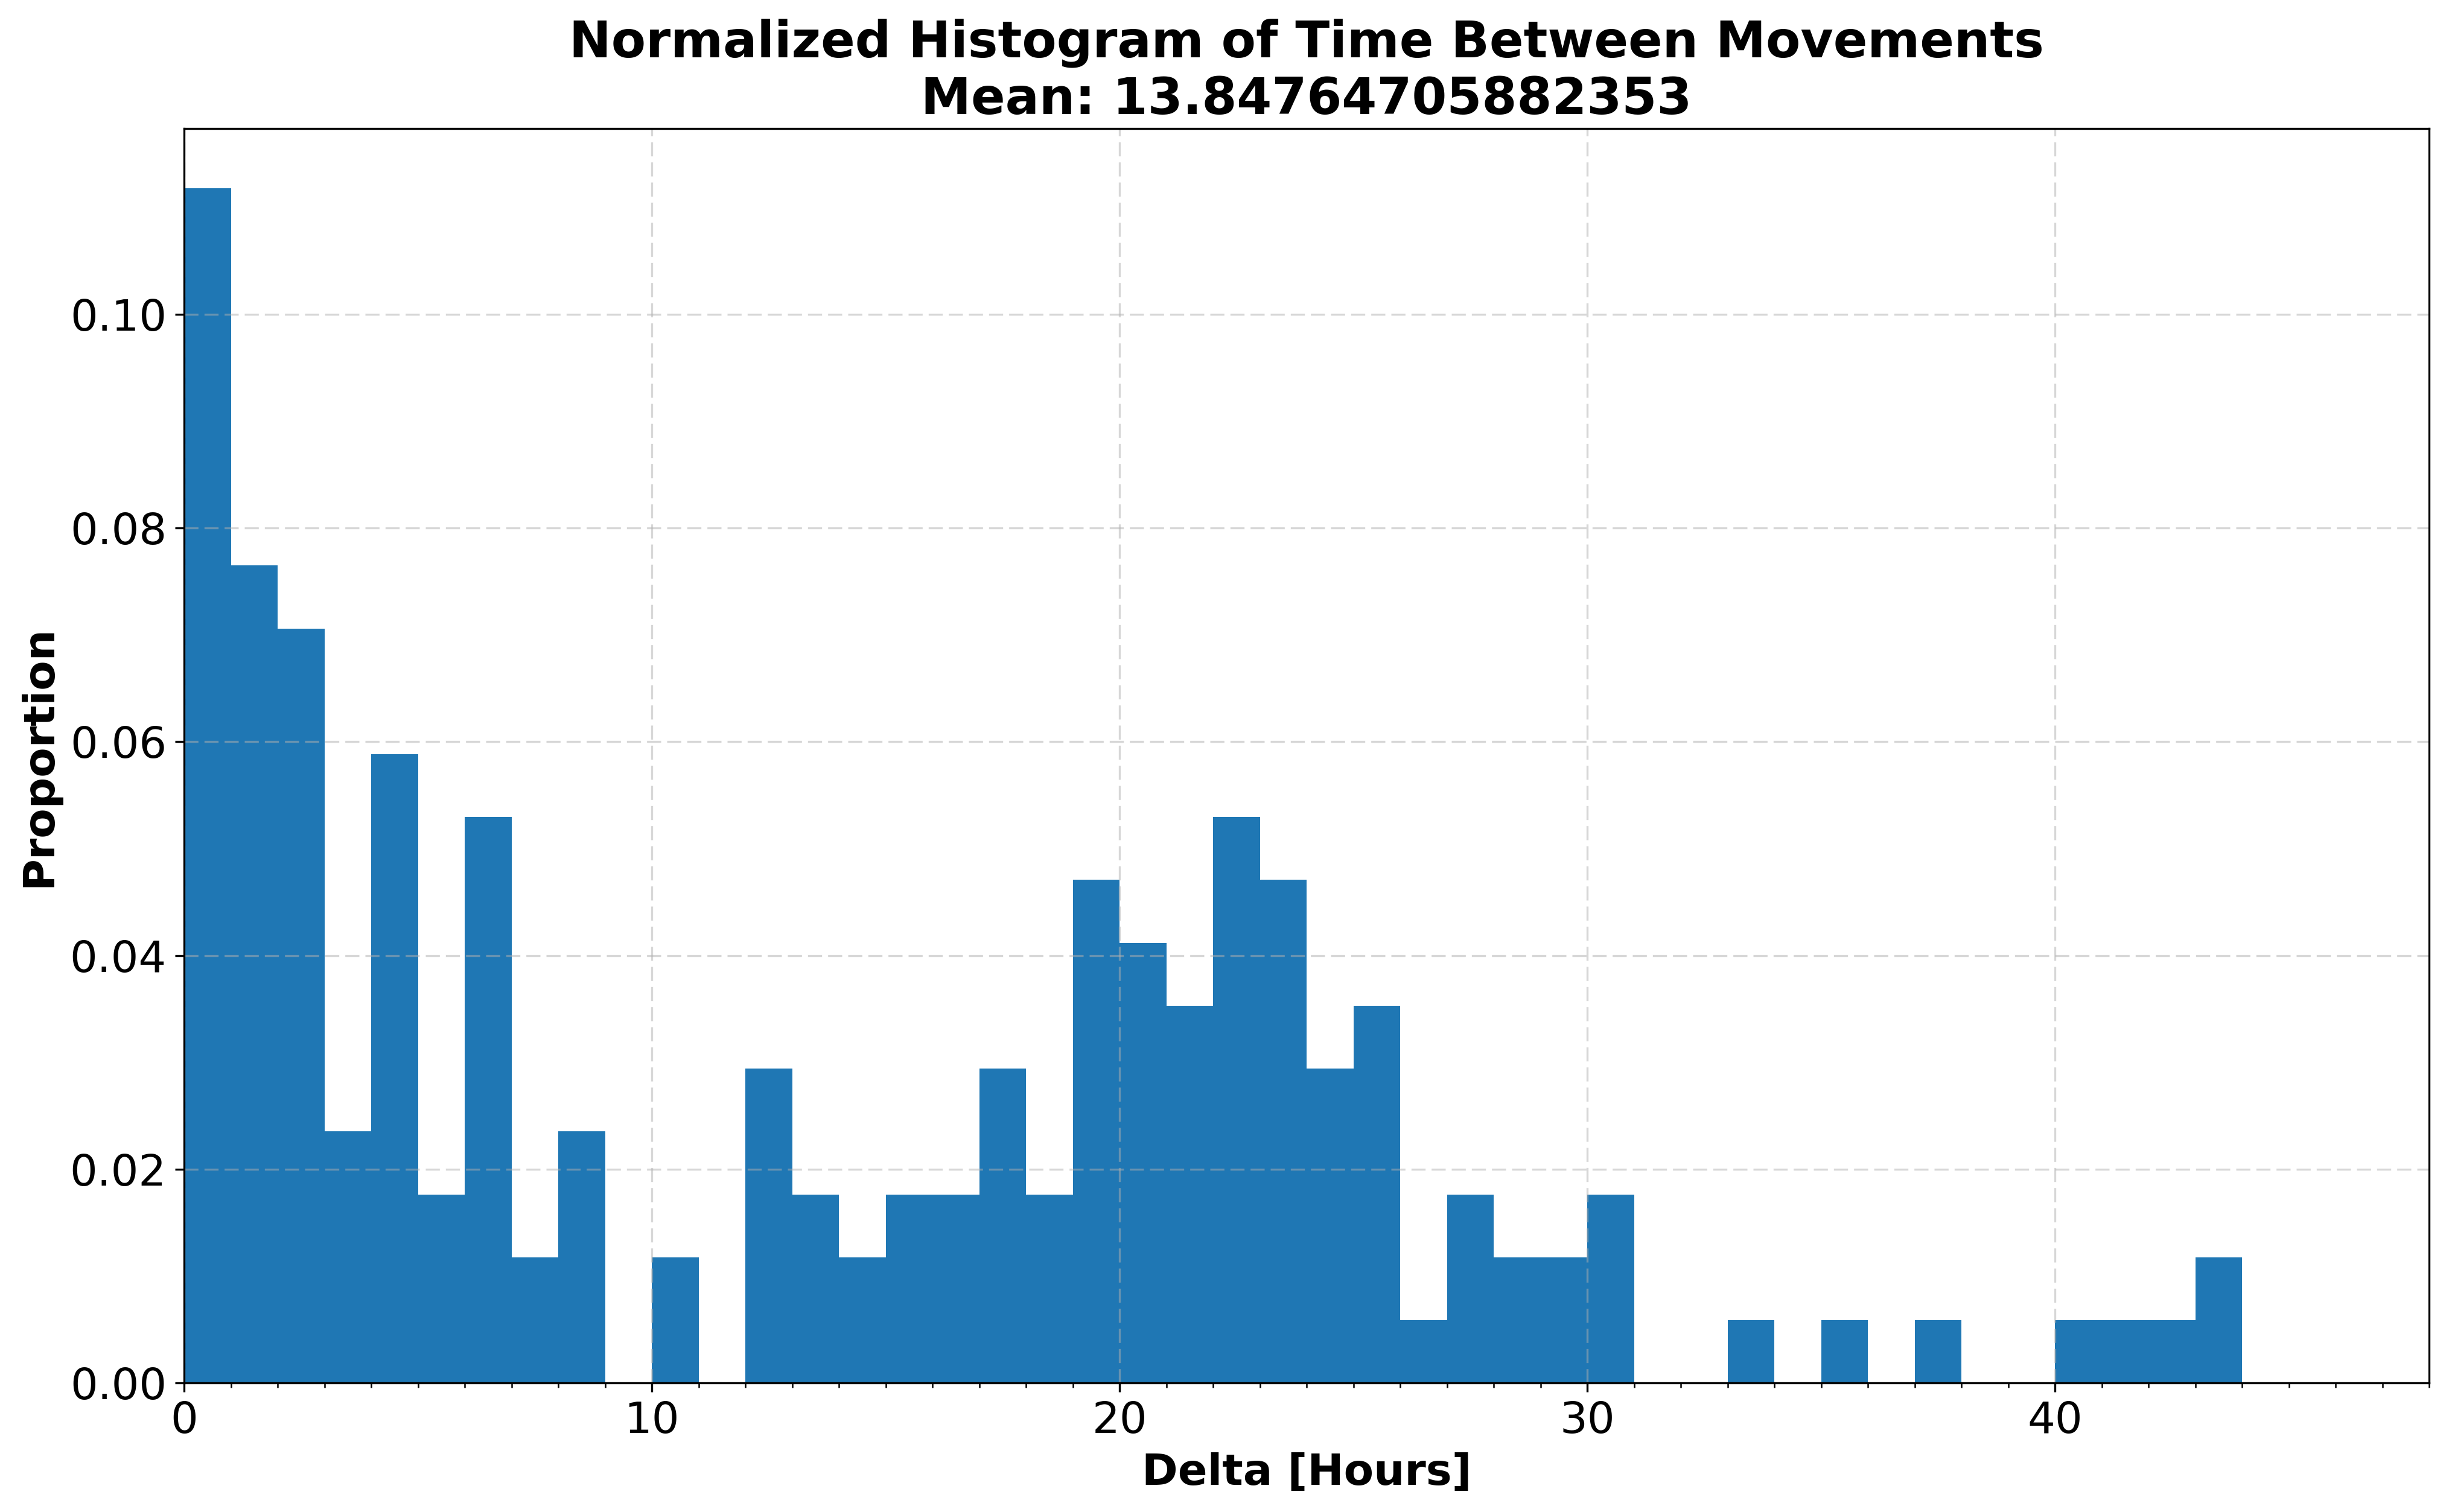
\includegraphics[width=\columnwidth]{time_between_movements.png}
    \caption{Distribution of Time Between Bowel Movements}\label{fig:time_between_movements}
\end{figure}


Bristol Stool Score (BSS) [TODO cite] of movement.

Health Quality Index plots by week are presented below.

\begin{figure}[t]
    \centering
    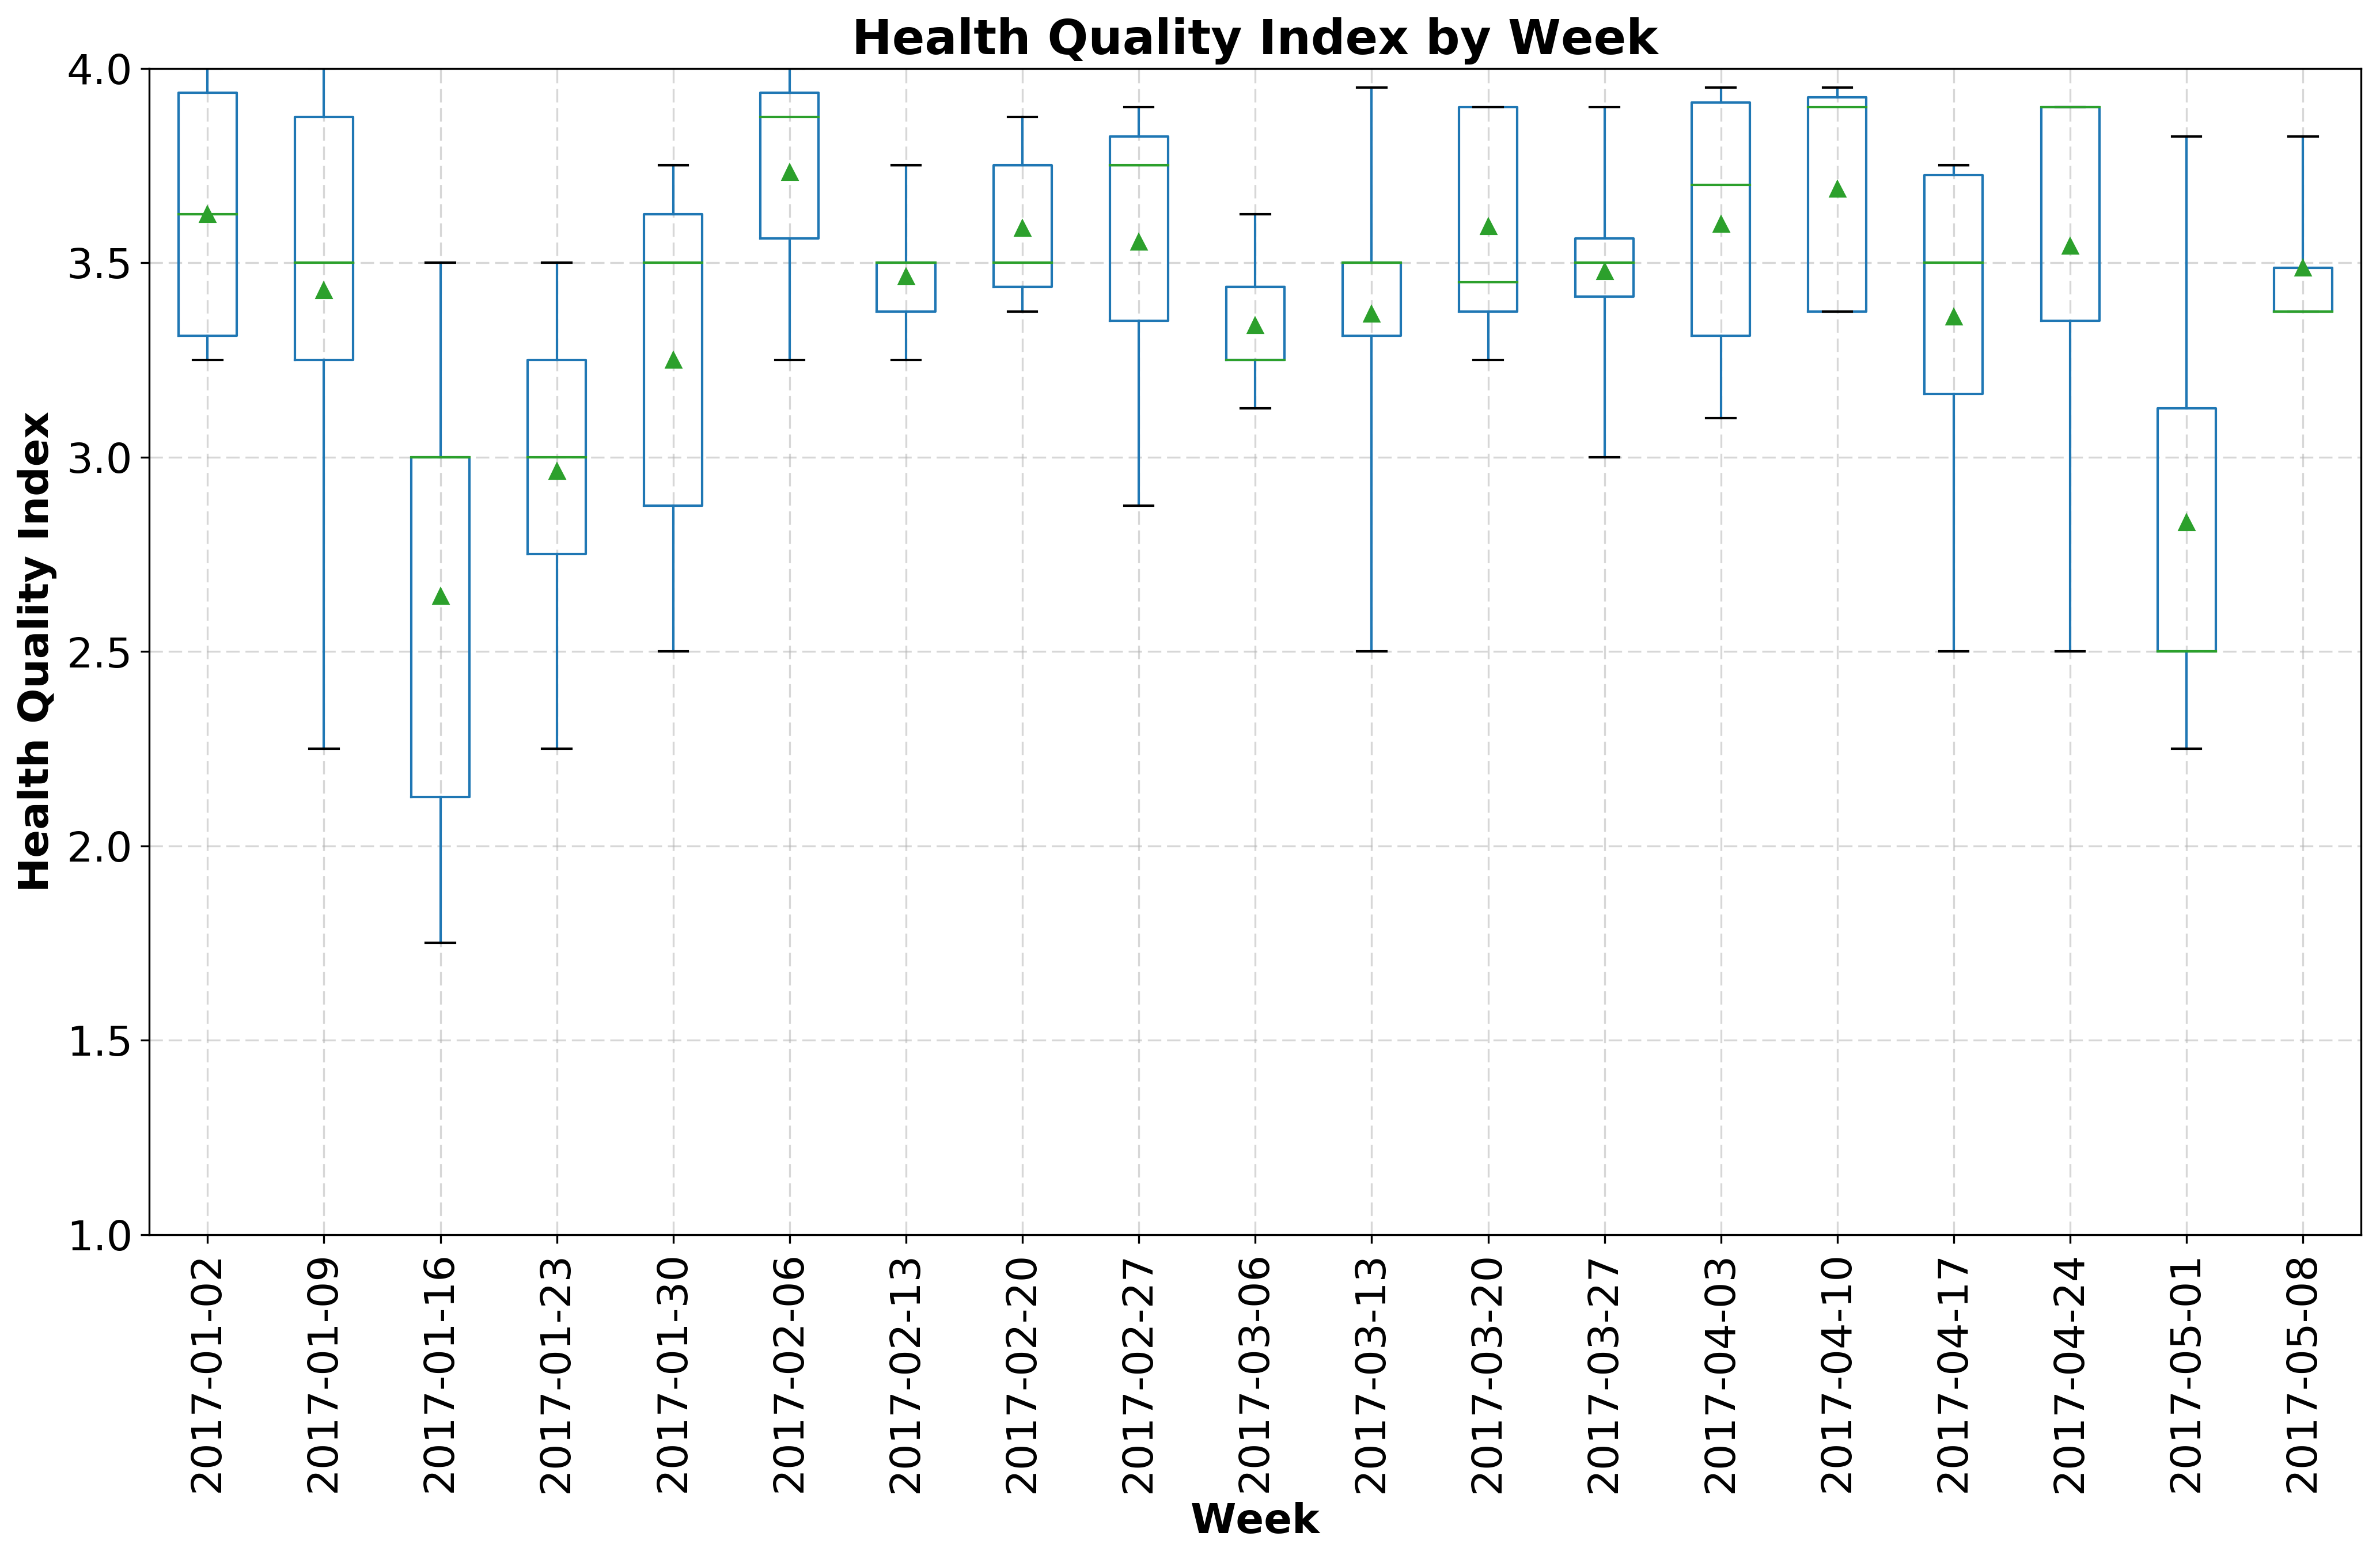
\includegraphics[width=\columnwidth]{hqi_box.png}
    \caption{Health Quality Index by Week}\label{fig:hqi}
\end{figure}

Mean minutes of cardio per week

Mean dosage of medicines per week

Mena daily weight per week

At date TODO, a full metaboloic panel was conducted with no anomolous results.


\section{Analysis}

A total of TODO days of daily recorrds were recorded which resulted in TODO BMs recorded.  The recorded time period is January 1, 2017 to TODO.  An exploratory analysis of the data follows.

We perform ordinary least squares (OLS) regresion using the data above to assess how medications and cardio affect HQI and BSS means on two different scales, 3 days and 7 days.  Two different time scales are assessed allowing a degree of freedom for the treatments to reach therapeutic level when initiated and washout when discontinued.

With width specified:

TODO Verify and notate that all regression had signifiant p-value of f stat.

\begin{center}
    \begin{tabular}{ | l | r | r | r | r |}
    \hline
    \multicolumn{5}{ |c| }{Regressor: HQI 3-Day Mean} \\
    \hline
     & coef & std err & t & $P>\left|t\right|$ \\ \hline
    Intercept & 3.1799 & 0.081 & 39.273 & 0.000    \\
    cardio [hrs]    &-0.0737     & 0.046     &-1.604     & 0.113\\
    nexium [20mg]    &     0.1697 &     0.053  &    3.206  &    *0.002\\
    librax [capsule]   &     0.0642 &     0.034  &    1.896  &    0.062\\
    clartin-d [capsule]    &    -0.0975 &     0.083  &   -1.178  &    0.243\\
    vitamin d [5000IU]     &    -0.0163 &     0.015  &   -1.105  &    0.272\\
    Metamucil [serving]     &    -0.0518 &     0.084  &   -0.615  &    0.540 \\
    \hline
    \end{tabular}
\end{center}

\begin{center}
    \begin{tabular}{ | l | r | r | r | r |}
    \hline
    \multicolumn{5}{ |c| }{Regressor: HQI 7-Day Mean} \\
    \hline
     & coef & std err & t & $P>\left|t\right|$ \\ \hline
    Intercept & 3.1799 & 0.081 & 39.273 & 0.000    \\
    cardio [hrs]    &-0.0737     & 0.046     &-1.604     & 0.113\\
    nexium [20mg]    &     0.1697 &     0.053  &    3.206  &    *0.002\\
    librax [capsule]   &     0.0642 &     0.034  &    1.896  &    0.062\\
    clartin-d [capsule]    &    -0.0975 &     0.083  &   -1.178  &    0.243\\
    vitamin d [5000IU]     &    -0.0163 &     0.015  &   -1.105  &    0.272\\
    Metamucil [serving]     &    -0.0518 &     0.084  &   -0.615  &    0.540 \\
    \hline
    \end{tabular}
\end{center}

We see from Table TODO and TODO that on 3-day time scales, TODO is statistically signifiant and on week-long time scales, TODO is statistically significant.

We regress on the number of abnormal movements of both 3 day and 7 day in the future.

\begin{center}
    \begin{tabular}{ | l | r | r | r | r |}
    \hline
    \multicolumn{5}{ |c| }{Regressor: Abnormal Events 3-Day Mean} \\
    \hline
     & coef & std err & t & $P>\left|t\right|$ \\ \hline
    Intercept & 3.1799 & 0.081 & 39.273 & 0.000    \\
    cardio [hrs]    &-0.0737     & 0.046     &-1.604     & 0.113\\
    nexium [20mg]    &     0.1697 &     0.053  &    3.206  &    *0.002\\
    librax [capsule]   &     0.0642 &     0.034  &    1.896  &    0.062\\
    clartin-d [capsule]    &    -0.0975 &     0.083  &   -1.178  &    0.243\\
    vitamin d [5000IU]     &    -0.0163 &     0.015  &   -1.105  &    0.272\\
    Metamucil [serving]     &    -0.0518 &     0.084  &   -0.615  &    0.540 \\
    \hline
    \end{tabular}
\end{center}

\begin{center}
    \begin{tabular}{ | l | r | r | r | r |}
    \hline
    \multicolumn{5}{ |c| }{Regressor: Abnormal Events 7-Day Mean} \\
    \hline
     & coef & std err & t & $P>\left|t\right|$ \\ \hline
    Intercept & 3.1799 & 0.081 & 39.273 & 0.000    \\
    cardio [hrs]    &-0.0737     & 0.046     &-1.604     & 0.113\\
    nexium [20mg]    &     0.1697 &     0.053  &    3.206  &    *0.002\\
    librax [capsule]   &     0.0642 &     0.034  &    1.896  &    0.062\\
    clartin-d [capsule]    &    -0.0975 &     0.083  &   -1.178  &    0.243\\
    vitamin d [5000IU]     &    -0.0163 &     0.015  &   -1.105  &    0.272\\
    Metamucil [serving]     &    -0.0518 &     0.084  &   -0.615  &    0.540 \\
    \hline
    \end{tabular}
\end{center}

Tables TODO and TODO show statistically signifance for TODO and TODO.  Clariten-D has a signifitant effect on TODO day mean abnormal movements.  The coeffecient is postive meaning it increase the number of adverse events which is not desireable.  Clariten-D is not signifnitamnt in tables TODO and TODO and therefore we conclude is doesn't postively contrinute to HQI but postively contributes to the number of negative events.  The administration of Clariten-D was administrated during the period nexium and librax were adminstered.  The adverse events during this period prompted the author to contacted several doctors and describeb the problem and request a suggested cure.  All doctors suggested the librax was the main contributued and advised to reduce intake.  The author reduced the librax resulting in a slight increase in symptoms. The author then discontinued taking clariten-d and the symptoms resolved as predicted by the regression model.

\section*{Conclusion}
We demonstrate simple, lightweight daily tracking of medications, exercise, Bristol Stool Scores, and a Health Quality Index can be utilized to manage and reduce symptoms in an N=1 setting.  We demonstrate how simple staticial analysis can be used to tailor medical treatment for an individual allowing for the identification and resolution of bowel issues for an IBS-D patient.

% use section* for acknowledgment
\section*{Acknowledgment}
The authors would like to thank TODO for the useful discussions and reviews.

\IEEEtriggeratref{12}

% trigger a \newpage just before the given reference
% number - used to balance the columns on the last page
% adjust value as needed - may need to be readjusted if
% the document is modified later
%\IEEEtriggeratref{8}
% The "triggered" command can be changed if desired:
%\IEEEtriggercmd{\enlargethispage{-5in}}

% references section

% can use a bibliography generated by BibTeX as a .bbl file
% BibTeX documentation can be easily obtained at:
% http://mirror.ctan.org/biblio/bibtex/contrib/doc/
% The IEEEtran BibTeX style support page is at:
% http://www.michaelshell.org/tex/ieeetran/bibtex/
\bibliographystyle{./bib/IEEEtran}
% argument is your BibTeX string definitions and bibliography database(s)
\bibliography{./bib/IEEEabrv,./bib/dcbPaperDatabase}
%
% <OR> manually copy in the resultant .bbl file
% set second argument of \begin to the number of references
% (used to reserve space for the reference number labels box)
%\begin{thebibliography}{1}
%
%\bibitem{IEEEhowto:kopka}
%H.~Kopka and P.~W. Daly, \emph{A Guide to \LaTeX}, 3rd~ed.\hskip 1em plus
%  0.5em minus 0.4em\relax Harlow, England: Addison-Wesley, 1999.
%
%\end{thebibliography}




% that's all folks
\end{document}


